\documentclass[12pt,fleqn]{article}
\usepackage{fullpage}
\usepackage{amsmath}
\usepackage{multirow}
\usepackage{graphicx}
\usepackage{indentfirst}
\title{\LARGE \textbf{Trabajo práctico 2}}
\author{Martín Rossi}
\date{}
\begin{document}
\maketitle
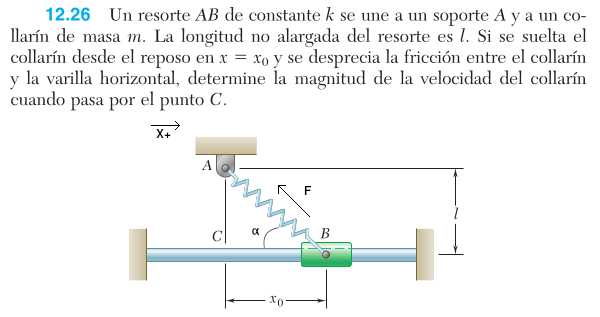
\includegraphics[width=\linewidth]{12.26}
\newpage
$F_R: \textrm{Fuerza del resorte}$

$F_R=-k*d=-k*(\sqrt{x^2+l^2}-l)$

\begin{align*}
  \sum{F_x}&=m*a\\
  F_R*cos(\alpha)&=m*a\\
  -k*(\sqrt{x^2+l^2}-l)*\frac{x}{\sqrt{x^2+l^2}}&=m*a\\
  -\frac{k}{m}*(\sqrt{x^2+l^2}-l)*\frac{x}{\sqrt{x^2+l^2}}&=a=v\frac{\delta v}{\delta x}\\
  -\frac{k}{m}*\int_{x_0}^0x-\frac{x*l}{\sqrt{x^2+l^2}}\delta x&=\int_0^{v_c}v\delta v\\
  -\frac{k}{m}*\frac{2*l*\sqrt{x_0^2+l^2}-x_0^2-2*l^2}{2}&=\frac{v_0^2}{2}\\
  -\frac{k}{m}*(2*l*\sqrt{x_0^2+l^2}-x_0^2-2*l^2)&=v_0^2\\
  \frac{k}{m}*(-2*l*\sqrt{x_0^2+l^2}+x_0^2+2*l^2)&=v_0^2\\
  \frac{k}{m}*(x_0^2+2*l^2-2*l*\sqrt{x_0^2+l^2})&=v_0^2\\
  \frac{k}{m}*(x_0^2+l^2-2*l*\sqrt{x_0^2+l^2}+l^2)&=v_0^2\\
  \frac{k}{m}*(\sqrt{x_0^2+l^2}-l)^2&=v_0^2\\
  \sqrt{\frac{k}{m}}*(\sqrt{x_0^2+l^2}-l)&=v_0
\end{align*}
\newpage
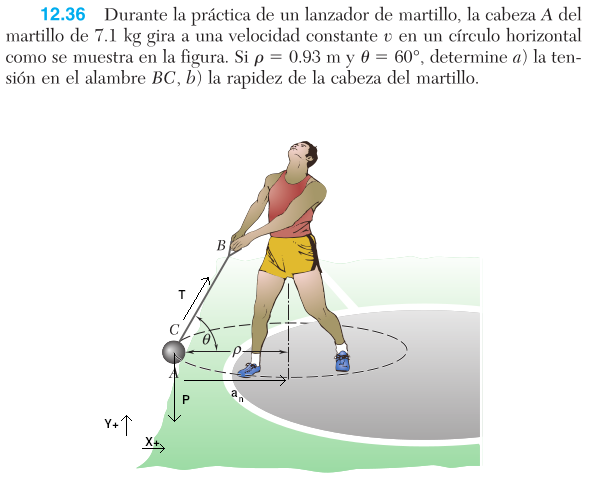
\includegraphics[width=\linewidth]{12.36}
\newpage
La única aceleración que experimenta el martillo es la componente normal $a_n$ porque se mueve con velocidad constante.\\

$\sum{F_y}=0$

$\sum{F_x}=m*a_n$

$\theta=60^\circ$

$\rho=0.93m$

$m=7.1kg$
\subsubsection*{a)}
\begin{align*}
  \sum{F_y}&=0\tag{el martillo no tiene aceleración vertical}\\
  P-T*\textrm{sin}(60)&=0\\
  69.58-T*0.87&=0\\
  T&=80.34N
\end{align*}
\subsubsection*{b)}
\begin{align*}
  \sum{F_x}&=m*a_n\tag{sumatoria de fuerzas en el eje x}\\
  T*\textrm{cos}(60)&=m*\frac{v^2}{\rho}\\
  80.34*0.5&=7.1*\frac{v^2}{0.93}\\
  v&=2.39m/seg
\end{align*}
\newpage
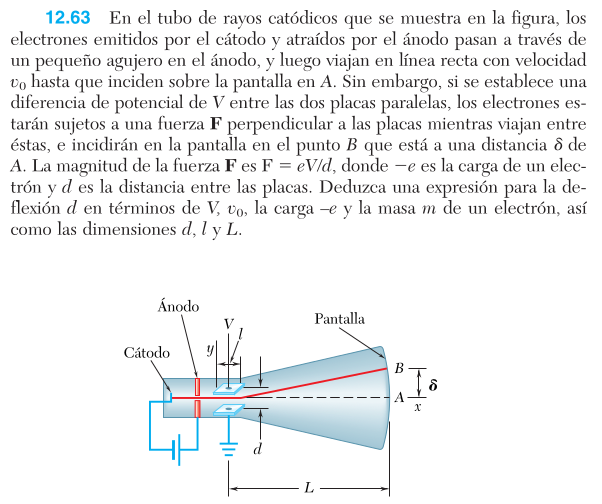
\includegraphics[width=\linewidth]{12.63}
\newpage
\[t_l=\frac{l}{v_0}\tag{tiempo que le toma al electrón recorrer las placas}\]

\[\sum{F_y}=m*a_y\tag{sumatoria de fuerzas en el eje y}\]
\[\frac{e*V}{d}=m*a_y\]
\[\frac{e*V}{d*m}=a_y\]

\[y_l=\frac{a}{2}*t_l^2=\frac{e*V}{2*d*m}*\frac{l^2}{v_0^2}\tag{distancia en y cuando sale de las placas}\]

\[v_l=a_y*t_l=\frac{e*V*l}{d*m*v_0}\tag{velocidad en y cuando sale de las placas}\]

\begin{align*}
  \delta&=y_l+v_l*t_{L-l}\\
        &=\frac{e*V}{2*d*m}*\frac{l^2}{v_0^2}+\frac{e*V*l}{d*m*v_0}*\frac{L-\frac{l}{2}}{v_0}\\
        &=\frac{e*V*l^2}{2*d*m*v_0^2}+\frac{e*V*l*(L-\frac{l}{2})}{d*m*v_0^2}\\
        &=\frac{e*V*l^2+2*e*V*l*(L-\frac{l}{2})}{2*d*m*v_0^2}\\
        &=\frac{e*V*l^2+2*e*V*l*L-e*V*l^2}{2*d*m*v_0^2}\\
        &=\frac{e*V*l*L}{d*m*v_0^2}
\end{align*}
\end{document}